\documentclass[12pt]{article}
\usepackage[T1]{fontenc}
\usepackage[latin9]{luainputenc}
\usepackage{geometry}
\geometry{verbose,tmargin=0.8in,bmargin=0.8in,lmargin=0.7in,rmargin=0.7in}
\usepackage{color}
\usepackage{babel}
\usepackage{float}
\usepackage{amsmath}
\usepackage{amsthm}
\usepackage{amssymb}
\usepackage{graphicx}
\usepackage{setspace}
\usepackage[authoryear]{natbib}
\usepackage{longtable}
\usepackage{ltablex}
\onehalfspacing
\usepackage[unicode=true,pdfusetitle,
            bookmarks=true,bookmarksnumbered=false,bookmarksopen=false,
 breaklinks=false,pdfborder={0 0 1},backref=false,colorlinks=true]
 {hyperref}
\hypersetup{
 pdfborderstyle=,pdfborderstyle={},pdfborderstyle={},linkcolor=blue,urlcolor=blue,citecolor=blue,pdfstartview={FitH},hyperfootnotes=false}
 \setlength{\arrayrulewidth}{0.5mm}
 \setlength{\tabcolsep}{18pt}
\makeatletter
% \usepackage{subcaption}


% \usepackage{caption}
% \usepackage{subcaption}

%%%%%%%%%%%%%%%%%%%%%%%%%%%%%% LyX specific LaTeX commands.
%% Because html converters don't know tabularnewline
\providecommand{\tabularnewline}{\\}

%%%%%%%%%%%%%%%%%%%%%%%%%%%%%% User specified LaTeX commands.
\usepackage{etex}
%\usepackage[round,longnamesfirst]{natbib}
\usepackage{amsfonts}
\usepackage{mathpazo}
\usepackage{hyperref}
\usepackage{xcolor}
\hypersetup{
	colorlinks,
	linkcolor={blue!75!black},
	citecolor={blue!75!black},
}
\usepackage{multimedia}
\usepackage{graphicx, color}
%\usepackage{pstricks,pst-node,fancybox,pst-text}
\usepackage{epsfig}
\usepackage{amsthm}
\usepackage{mathtools}
\usepackage{esint}
\usepackage{amssymb}
\usepackage{url}
\usepackage{graphicx,subfig}
\usepackage{relsize}
\usepackage{amsfonts}
\usepackage{fancyheadings}
\usepackage{float}
\usepackage{color}
\usepackage{mathrsfs}
\usepackage{setspace}
%\usepackage{lipsum}
%\usepackage{tikz}
\usepackage[mathscr]{euscript}
\usepackage{caption}
%\usepackage{subcaption}
\usepackage{pdflscape}
\usepackage{rotating}
\usepackage{booktabs}
%\usepackage[utf8]{inputenc}
\usepackage[T1]{fontenc}
\usepackage{geometry}
\newtheorem{thm}{Theorem}[section]
\newtheorem{cor}[thm]{Corollary}
\newtheorem{lem}[thm]{Lemma}
\newtheorem{prop}[thm]{Proposition}
\usepackage[bottom]{footmisc}
\usepackage{enumerate} % for numbered lists

\newenvironment{definition}[1][Definition]{\begin{trivlist}
		\item[\hskip \labelsep {\bfseries #1}]}{\end{trivlist}}

\setlength{\topmargin}{-0.4in}
\setlength{\textheight}{8.85in}

%%  Edited to make stat review comments easier
\newif\ifStatReview% \StatReviewfalse
%%\StatReviewtrue    %   Show stat review comments
\StatReviewfalse    %   Ignore stat review comments
\ifStatReview
    \setlength{\oddsidemargin}{-0.2in}
    \setlength{\evensidemargin}{0.0in}
    \setlength{\textwidth}{6.0in}
    
    
    \usepackage{tikz}
    \let\oldmarginpar\marginpar
    % renew the \marginpar command to draw 
    % a node; it has a default setting which 
    % can be overwritten
    \renewcommand{\marginpar}[2][rectangle,draw,fill=yellow,rounded corners,text width=3.5cm]{%
            \oldmarginpar{%
            \tikz \node at (0,0) [#1]{#2};}%
            }
    \newcounter{statreview}
    \newenvironment{statreview}[1][]{\refstepcounter{statreview}\par\medskip
       \textbf{Stat Review~\thestatreview #1} \rmfamily}{\medskip}
  \else
    \setlength{\oddsidemargin}{-0.2in}
    \setlength{\evensidemargin}{0.0in}
    \setlength{\textwidth}{6.93in}
    \renewcommand{\marginpar}[2][]{}
\fi

\renewcommand{\baselinestretch}{1.44}

\usepackage{setspace}
\onehalfspacing

\@ifundefined{showcaptionsetup}{}{%
 \PassOptionsToPackage{caption=false}{subfig}}
\usepackage{subfig}
\makeatother


\begin{document}
\title{Title Goes Here!!!\thanks{Valdes-Bobes: University of Wisconsin.
		I thank [X] for helpful comments and discussions.}}
\author{Mitchell Valdes-Bobes}
\maketitle
\begin{abstract}
	We examine [X]
\end{abstract}
\thispagestyle{empty}

\pagebreak{}
This paper .... 

% \begin{figure}[!tph]
% 	\caption{Technological Change by Occupation \label{fig:Technology Adoption by firms}}
% 	\begin{centering}
% 		\subfloat[Computer \& software req. by occ.]{
% 			\centering{}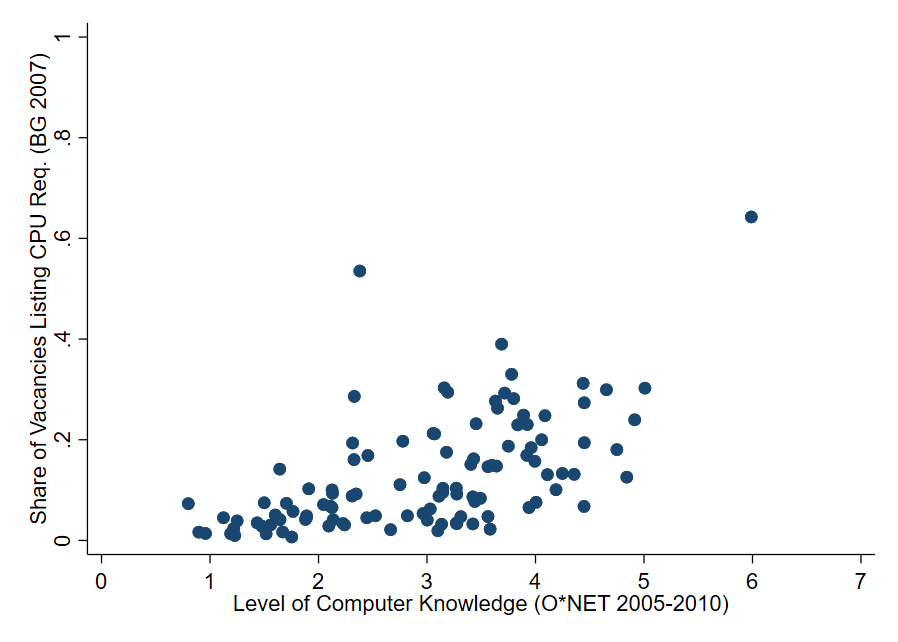
\includegraphics[width=8.5cm,height=8.5cm,keepaspectratio]{./images/scatter_level_BG_2007_ONET_15_1_pres_2021_08_18.png}}
% 		\subfloat[Changes in computer \& software req. by occ.]{
% 			\centering{}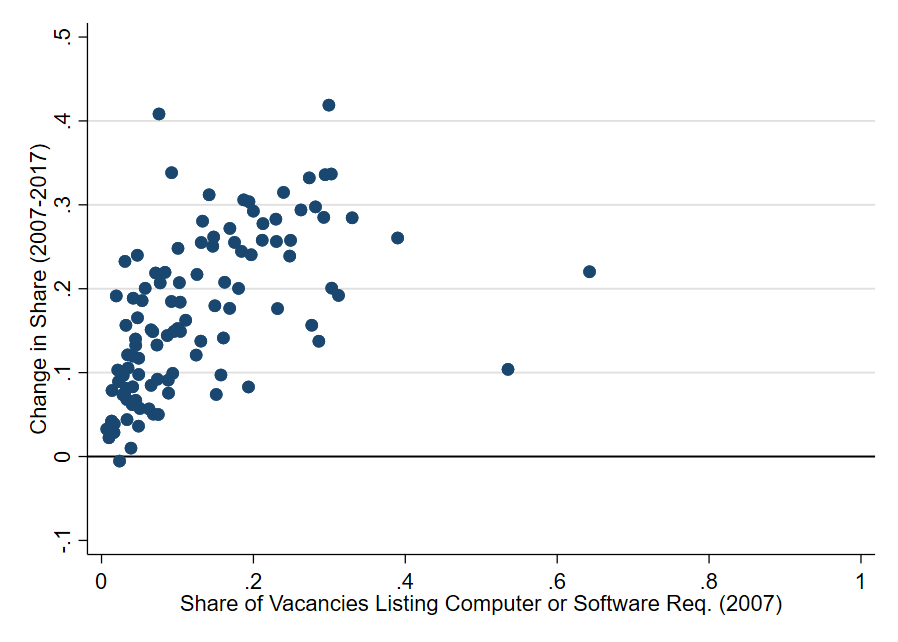
\includegraphics[width=8.5cm,height=8.5cm,keepaspectratio]{./images/scatter_chg_computer_by_initial_pres_2007_2021_08_18.png}}
% 		\par\end{centering}
% 	\emph{Notes: Panel (a) displays the level of knowledge in computers reported in O{*}NET (x-axis) and the share of vacancies listing a computer or software requirement by occupation as measured in the Burning Glass database in 2007 (y-axis). Panel (b) displays the share of vacancies listing a computer or software requirement by occupation in 2007 (x-axis), and the change in the share of vacancies listing a computer or software requirement between 2007 and 2017 (y-axis) as measured in the Burning Glass database. Occupations are measured using four-digit SOC codes.}\\	
% \end{figure}


\section{Introduction}\label{sec:introduction}

\section{Literature Review}\label{sec:literature_review}

\section{Industry Specific Skill Premium}

\section{Data}\label{sec:data}
I estimate the model following the approach outlined in KORV \citet{krusell2000capital}. I constructed data series for wages, labor input, and capital input from 1963 to \textcolor{red}{FINAL YEAR} to replicate KORV with updated data following \citet{ohanian2021revisiting}. I then collect the same series at the industry level to re-estimate the model, due to data availability industry series cover the period from \textcolor{red}{INITIAL YEAR}-\textcolor{red}{FINAL YEAR}.

Labor input and wages are estimated using CPS data downloaded from IPUMS, see \citet{flood2015integrated}, 

\subsection{Capital Data}\label{sec:capital_data}
To extend both capital series to replicate KORV I obtained investment series in equipment $(I_e)$ and structures $(I_s)$ from NIPA Table 5.2.5. Then the equipment $(K_e)$ and structure $(K_s)$ capital series were constructed using the perpetual inventory method:
\begin{equation}\label{eq:capital_law_motion}
  K_{i_{t+1}} = (1 - \delta_{i_t}) K_{i_{t}} + I_{i_{t}} \qquad i\in\{e, s\}
\end{equation}
\noindent
I departed from KORV by using time-varying depreciation rates $\delta_{i_t}$, instead of constant depreciation rates for each series. As in \citep{ohanian2021revisiting} I deflate structures using the implicit price deflator of GDP \footnote{Available \url{https://fred.stlouisfed.org/series/GDPDEF}}, and equipment using the product of the consumption delfator\footnote{Available at \url{https://fred.stlouisfed.org/series/CONSDEF}} and the relative price of equipment \footnote{Available at \url{https://fred.stlouisfed.org/series/PERIC}}. 

To obtain capital data at the industry level I used the BEA Fixed Assets dataset to obtain investment and capital consumption series by industry and type, details of which tables were used are included in Appendix \ref{subsec:capital-inputs-labor-share}. Fixed Assets dataset groups industries into 76 groups. To construct a series of the labor share of output by industry, I used the BEA-BLS Integrated Industry-level Production Accounts (KLEMS)\footnote{Available at \url{https://www.bls.gov/productivity/articles-and-research/industry-production-account-capital.xlsx}}. KLEMS data consists on 57 industry groups some of which are aggregations of industries on the BEA dataset. Table %\ref{tab: changes_by_occ} 
presents the crosswalk between BEA, KLEMS, and Census industry codes. I used the crosswalk provided by \citep{acemoglu2020unpacking}. A description of the codes is in \textcolor{red}{INSER TABLE AND REFERENCEIT}.

\subsection{Labor Data}\label{sec:labor_data}

\section{Model}\label{sec:model}
This section presents the model which is the same as \citep{krusell2000capital}. There are four inputs for production in this economy: two types of capital, equipment $(k_e)$ and structures $(k_s)$ and two types of labor, skilled $(s)$ and unskilled $(u)$. Inputs are combined thourgh a produciton funciton $G(\cdot)$ to produce three final goods: consumption $(c)$, investment in equipment $(i_e)$ and investment in structures $(i_s)$. Assuming an hicks-newutral technological shocks $A$, the aggreate production is given by
\begin{equation}\label{eq:production}
  c_t + i_{e_t} + i_{s_t} = Y_t =  A_t G(k_{s_t}, k_{e_t}, u_t, s_t)
\end{equation}
Capital evelves following the law of miotion in \eqref{eq:capital_law_motion}. The production function is assumed to be Cobb-Douglas in structures and a nested CES in all other inputs:
\begin{equation}\label{eq:production_fun}
  G(k_{s_t}, k_{e_t}, u_t, s_t) = k_{s_t}^\alpha\left( \mu u_t^\sigma + (1-\mu)\left(\lambda k_{s_t}^\rho (1-\lambda)s_t^\rho\right)^\frac{\sigma}{\rho}\right)^\frac{1-\alpha}{\sigma}
\end{equation}
where $\alpha$ is the share of capital structures in output, $\mu$  and $\lambda$  are income shares, $\rho$ and $\sigma$ govern the elasticity of substitution between capital equipment and labor:
\begin{itemize}
  \item $\sigma_{H} = 1/(1-\rho)$ is the elasticity of substitution between equipment and high-skilled.
  \item $\sigma_{L} = 1/(1-\sigma)$ is the elasticity of substitution between low-skilled and equipment + high skill labor.
\end{itemize}
Labor input is defined as 
\begin{align*}
  u &= \psi^u_t h^u_t\\
  s &= \psi^s_t h^s_t
\end{align*}
where $\psi^i_t$ is the (unobserved) efficiency of each type of labor and $h^i_t$ is the number of labor hours. 

\subsection{Skill Premium}
The model can be used to analyze the determinants of the skill premium growth, i.e. growth of  the ratio of wages of skilled labor to wages of unskilled labor. 

Firms solve the following profit maximization problem 
\begin{equation}\label{eq:profit_max}
  \max_{k_{s_t}, k_{e_t}, u_t, s_t} G(k_{s_t}, k_{e_t}, u_t, s_t) - r_{s_t}k_{s_t} - r_{e_t}k_{e_t} - w_{u_t} h_{u_t} - w_{s_t} h_{s_t}
\end{equation}
$r_{s_t}$ and $r_{e_t}$ are rental rates of capital and  $w_{u_t}$ and $w_{s_t}$ are wages of unskilled and skilled workers. Assuming perfect competition, labor is payed it marginal productivity therefore the skill premium at time $t$, ($\omega_t$) is given by
\begin{equation}
  \omega_t = \frac{w_{s_t}}{w_{u_t}} = \frac{G_{h_s}(k_{s_t}, k_{e_t}, u_t, s_t) }{G_{h_u}(k_{s_t}, k_{e_t}, u_t, s_t) }
\end{equation}

this gives the following expression for the skill premium:

\begin{equation}\label{eq:skill_premium}
  \omega_{t}=\frac{(1-\mu)(1-\lambda)}{\mu}\left[\lambda\left(\frac{k_{e_t}}{s_{t}}\right)^{\rho}+(1-\lambda)\right]^{(\sigma-\rho) / \rho}\left(\frac{h_{u_t}}{h_{s_t}}\right)^{1-\sigma}\left(\frac{\psi^s_t}{\psi^u_t}\right)^{\sigma} .
\end{equation}
Since the object of interest is the steady state growth of $\omega_t$\eqref{eq:skill_premium} can be log-linearized to  obtain the following expression:
\begin{equation}\label{eq:skill_premium_log_linear}
  \ln \omega_{t} \simeq \lambda \frac{\sigma-\rho}{\rho}\left(\frac{k_{e_t}}{s_{t}}\right)^{\rho}+(1-\sigma) \ln \left(\frac{h_{u_t}}{h_{s_t}}\right)+\sigma \ln \left(\frac{\psi^s_t}{\psi^u_t}\right)
\end{equation}
Which in turn can be written in terms of growth rates:
\begin{equation}\label{eq:skill_premium_growth_rates}
  \begin{aligned}
    g_{\omega t} \simeq &(1-\sigma)\left(g_{h_{u_t}}-g_{h_{s_t}}\right)+\sigma\left(g_{\psi^s_t}-g_{\psi^u_t}\right) \\
    &+(\sigma-\rho) \lambda\left(\frac{k_{e_t}}{s_{t}}\right)^{\rho}\left(g_{k_{e_t}}-g_{h_{s_t}}-g_{\psi^s_t}\right) .
    \end{aligned}
\end{equation}
where $g_x$ denotes the growth rate of variable $x$, details on the derivations are include in Appendix~\ref{sec:derivations}. Equation~\eqref{eq:skill_premium_growth_rates} has the nice property that it is a linear combination of the growth rates of the inputs in the production function, this allows us to decompose the growth rate of the skill premium into three components that are easy to analyze:
\begin{enumerate}[(i)]
  \item $(1-\sigma)(g_{h_{u_t}}-g_{h_{s_t}})$ depends on the growth rate of one type of labor over the other. We assume that both types of labor are substitutes i.e $\sigma_L < 0 \implies (1-\sigma) < 0$ . This means that if skilled labor grows at a faster rate than unskilled labor,will decrease the skill-premium.
  \item $\sigma\left(g_{\psi^s_t}-g_{\psi^u_t}\right)$ depends on the growth rate of the productivity of one type of labor over the other. I follow \citep{krusell2000capital} in making the following stochastic assumptions about labor labor productivity:
  \begin{equation}\label{eq:stochastic_labor_productivity}
    \psi^i_t = \psi^i_0 + \epsilon \qquad \epsilon \sim N(0, \eta_\omega^2) \qquad i\in\{s,u\}
  \end{equation}
  This assumption guarantee that on average $\sigma (g_{\psi^s_t}-g_{\psi^u_t} )$ is constant over time and does not affect skill premium growth rate. 
  \item $(\sigma-\rho) \lambda\left(\frac{k_{e_t}}{s_{t}}\right)^{\rho}\left(g_{k_{e_t}}-(g_{h_{s_t}}+g_{\psi_{s_t}})\right)$ . This component depends on two factors:
  \begin{enumerate}
    \item The growth rate of equipment relative to the growth rates of skilled labor input. This allow us to characterize the capital-skill complementarity hypotesis as $\sigma > \rho$, if equipment capital grows faster than skilled labor, the skill-premium will increase.
    \item The ratio of capital equipment to efficiency units of skilled labor input (given our assumptions amounts to the growth rate of skilled labor input), this efect will get larger (smaller) over time if $\rho > 0\:$ ($\rho < 0$). 
  \end{enumerate}
\end{enumerate}

\section{Estimation}
I follow the same methodology as \citep{krusell2000capital} to estimate the model parameter. To simplify notation from now on I will refer to  the unobservable labor efficiencies as, $\psi_t = \{\psi^u_t, \psi^s_t\}$, the  inputs of the production function as $X_t = \{ k_{s_t} , k_{e_t}, h_{s_t}, h_{u_t}\}$ and the set of parameters to be estimated  as $\Phi  = \{\alpha, \sigma, \rho, \mu, \lambda, \psi^u_0, \psi^s_0, \eta_\omega \}$. 

Firms decide investment in structures based on expectations about future prices $q_{t+1}$. This is capture using a \textit{"no arbitrage"} condition, firms equate marginal returns on investment on  both types of capital. On the one hand marginal return on investment in capital structures is given by given by the sum of the marginal product of structures in $t+1$, $A_{t+1} G_{k_s}(X_{t+1}, \psi_{t+1} \mid \Phi )$ and undepreciated structures on $(1-\delta_s)$. On the other hand marginal return on investment in equipment is given by the sum of the marginal product of equipment in nexrt period, $q_t A_{t+1} G_{k_s}(X_{t+1}, \psi_{t+1} \mid \Phi )$  and depreciated structures $\mathbb{E}(q_t/q_{t+1})(1-\delta_e)$ the term $\mathbb{E}(q_t/q_{t+1})$, as in \citep{krusell2000capital} I make the simplifying assumption of 
$(1-\delta_e)\mathbb{E}(q_t/q_{t+1}) =(1-\delta_e)(q_t/q_{t+1}) + \nu_t$ where $\nu_t$ is normaly distributed with mean zero and variance $\eta_\nu^2$ this parameter is calibrated using dataonm $q_t$.\footnote{Since I use the same series of relative prices than KORV I take their calibration of $\eta_\nu = 0.02$}. Putting everithing together we have the following equation:
\begin{equation}\label{eq:no_arbitrage}
  A_{t+1} G_{k_s}(X_{t+1}, \psi_{t+1} \mid \Phi ) = q_t A_{t+1} G_{k_s}(X_{t+1}, \psi_{t+1} \mid \Phi ) + (1-\delta_e)\left(\frac{q_t}{q_{t+1}}\right) + \nu_t
\end{equation}

The other two structural equations used to estimate the model compare the labor share observed in the data to labor share predicted by the model $lsh(X_{t+1}, \psi_{t+1} \mid \Phi )$ and the wage-bill ratio observed in the data to wage-bill ratio predicted by the model $wbr(X_{t+1}, \psi_{t+1} \mid \Phi )$:
\begin{align}
  \frac{w_{s_t}h_{s_t} + w_{u_t}h_{u_t} }{Y_t} &= lsh(X_{t}, \psi_{t} \mid \Phi ) \label{eq:labor_share}\\
  \frac{w_{s_t}h_{s_t}}{w_{u_t}h_{u_t}} &= wbr(X_{t}, \psi_{t} \mid \Phi ) \label{eq:wage_bill_ratio}
\end{align}

Since the parameters $\mu, \lambda, \psi^u_0, \psi^s_0$ act as scaling parameters, to estimate the model one must be fixed, I follow \citep{krusell2000capital} in fixing $\psi^s_0$, the initial value of the productivity of skilled labor. When replicating their result on a extend sample I choose to fix $\psi^u_0 = 6$ as in the original, but choose diferent variants when estimating each industry to improve the fitness. Fuinally the parameter $\eta_\omega$ is choosen to minimize distance between the skill premium in the data and the skill premium predicted by the model.

The estimation process is a simulated two-stage pseudo-maximum likelihood estimation (SPMLE) developed by \citep{white1996estimation}. Is reasonable that the choice of labor is influenced the productivity shocks therefore skilled and unkilled labor in treated as endogenous. 

To allow for the possible dependence of hours worked on shocks, we use the two-stage SPML developed by, which is similar in spirit to two-stage least squares. We treat skilled and unskilled labor input as endogenous. To deal with the endogeneity, labor input is projected onto a constant, current, and lagged stock of capital equipment and structures, the lagged relative price of equipment, and a trend. The model is estimated using the instrumented labor input series, the series of capital and prices as the inputs of the model.

The the next stage we proceed as follows: taking the variance $\eta_\omega$ as given, for each date $t$ generate $S$ realizations the stochastic components of the model $\quad \varphi_t$ use those as inputs to generate $S$ realization of the structural equaitons \eqref{eq:no_arbitrage}, \eqref{eq:labor_share} and \eqref{eq:wage_bill_ratio}, to simplify notaiton I refer to each of those values as $\tilde{Z}^{i}_t(X_{t}, \psi_{t} \mid \Phi)$, (note that this is a vector of three values, one for each of the equations). Using the simulated data we obtain the first and second moments of the model: 
\begin{equation}\label{eq:first_moment}
  m(X_{t}, \psi_{t} \mid \Phi) = \frac{1}{S}\sum_{i=1}^S \tilde{Z}^{i}_t(X_{t}, \psi_{t} \mid \Phi)
\end{equation}
and
\begin{equation}\label{eq:second_moment}
  V(X_{t}, \psi_{t} \mid \Phi) = \frac{1}{S-1}\sum_{i=1}^S \left( \tilde{Z}^{i}_t(X_{t}, \psi_{t} \mid \Phi) - m(X_{t}, \psi_{t} \mid \Phi) \right) \left( \tilde{Z}^{i}_t(X_{t}, \psi_{t} \mid \Phi) - m(X_{t}, \psi_{t} \mid \Phi) \right)'
\end{equation}
Finally, we minimize same objective function as \citep{krusell2000capital}:
\begin{equation}\label{eq:objective_funct_estimation}
  \begin{aligned}
    \ell\left(Z^{T} ; X_{t}, \psi_{t} \mid \Phi\right)=&-\frac{1}{2 T} \sum_{t=1}^{T}\left\{\left[Z_{t}-m_{S}\left(\tilde{X}_{t} ; \phi\right)\right]^{\prime}\left(V_{S}\left(\tilde{X}_{t} ; \phi\right)\right)^{-1}\left[Z_{t}-m_{S}\left(\tilde{X}_{t} ; \phi\right)\right]\right.\\
    &\left.-\log \operatorname{det}\left(V_{S}\left(\tilde{X}_{t} ; \phi\right)\right)\right\}
    \end{aligned}    
\end{equation}
where $Z_{t}$ is the vector of model counterparts of $\tilde{Z}^{i}_t(X_{t}, \psi_{t} \mid \Phi)$.
\section{Results}\label{sec:results}
This section present the results of the estimation process. I first show the result of the replication of KORV for different time periods and  then summarize the results of the estimating the model for each industry.
\subsection{KORV Replication}\label{sec:results_original}
Table \ref{tab:estimation_korv} compares the results botained by \citep{krusell2000capital} to this replication using their 
original data ($1963$ - $1992$) \footnote{Available at Gianluca Violante's web-site: \url{http://violante.mycpanel.princeton.edu/Journals/Data_KORV.txt}}. I present also the estimation on the extended sample ($1963$ - $2018$) and on the subset of the extended sample for which there is coverage at the industry level  ($1988$ - $2018$). 

\begin{table}[h]
\begin{center}
  \begin{tabular}{rrrrr}
  \hline\hline
   & \textbf{KORV Estimation} & \textbf{Replication} & \textbf{Updated Data} & \textbf{Updated Data} \\
   & \texttt{$1963$ - $1992$} & \texttt{$1963$ - $1992$} & \texttt{$1963$ - $2018$} & \texttt{$1988$ - $2018$} \\\hline
  $\alpha$ & 0.117 & 0.113 & 0.118 & 0.08 \\
  $\sigma$ & 0.401 & 0.464 & 0.503 & 0.313 \\
  $\rho$ & -0.495 & -0.56 & -0.343 & -0.154 \\
  $\eta_\omega$ & 0.043 & 0.043 & 0.083 & 0.043 \\\hline\hline
\end{tabular}

  \caption{\label{tab:estimation_korv} Parameter estimates KORV model.}
\end{center}
\end{table}
Figures 


% \begin{figure}
  % \centering
  % \begin{subfigure}%[b]{0.3\textwidth}
  %     \centering
  %     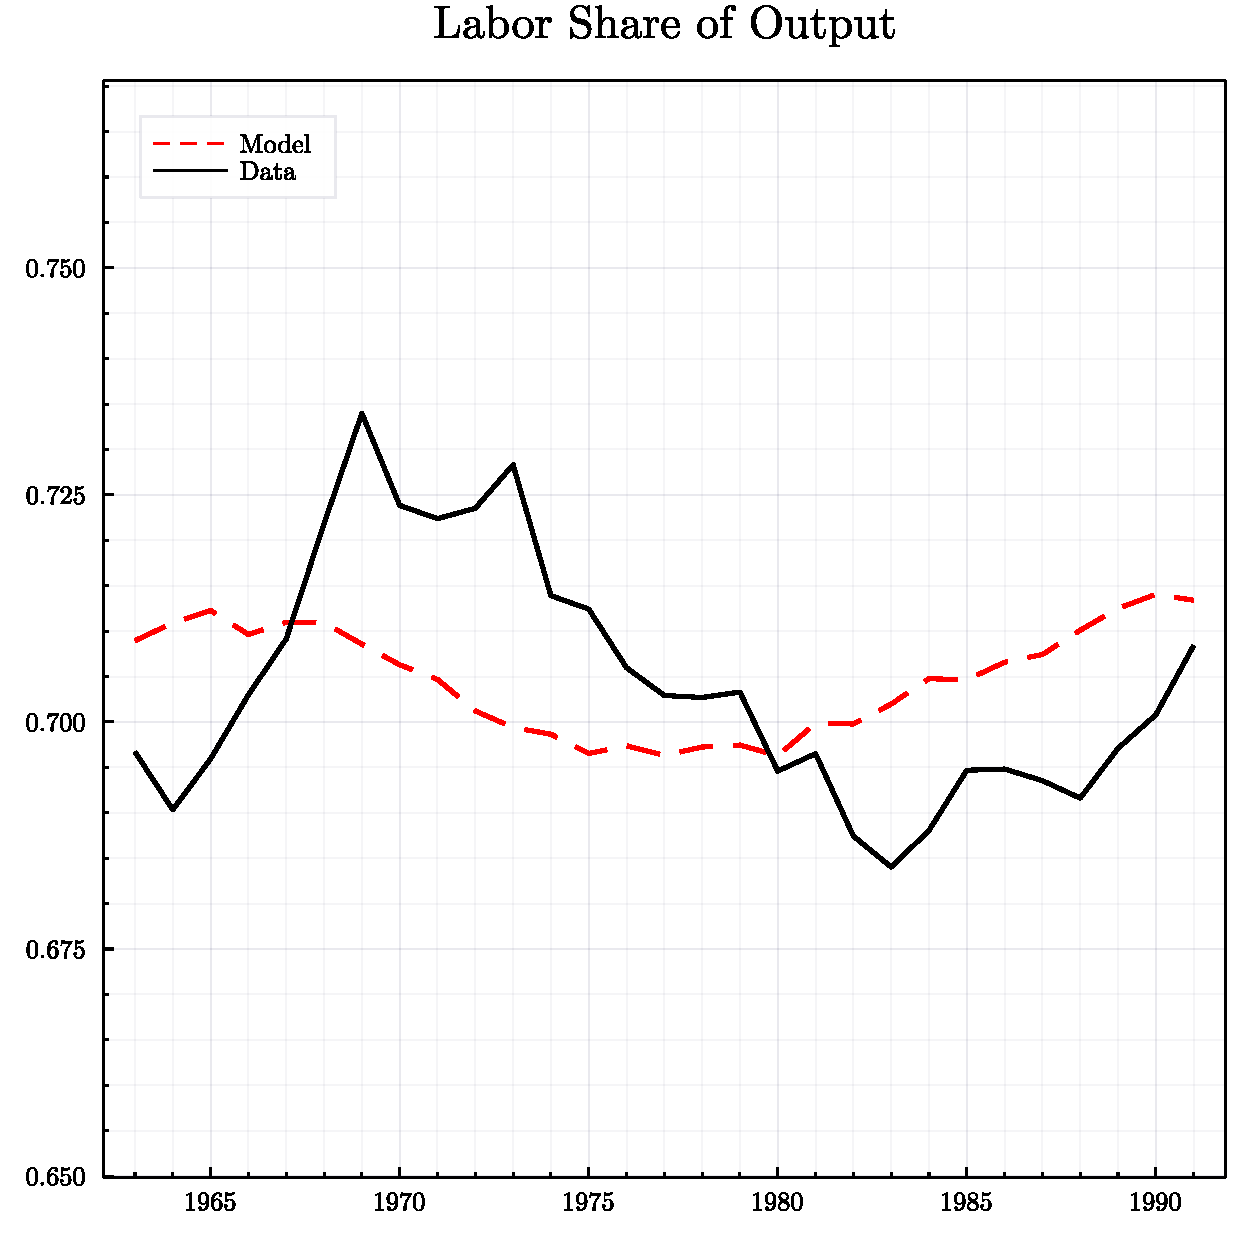
\includegraphics[width=\textwidth]{../images/fig:korv_estimation_ls_doc.pdf}
  %     \caption{$y=x$}
  %     \label{fig:y equals x}
  % \end{subfigure}
  % \hfill
  % \begin{subfigure}%[b]{0.3\textwidth}
  %     \centering
  %     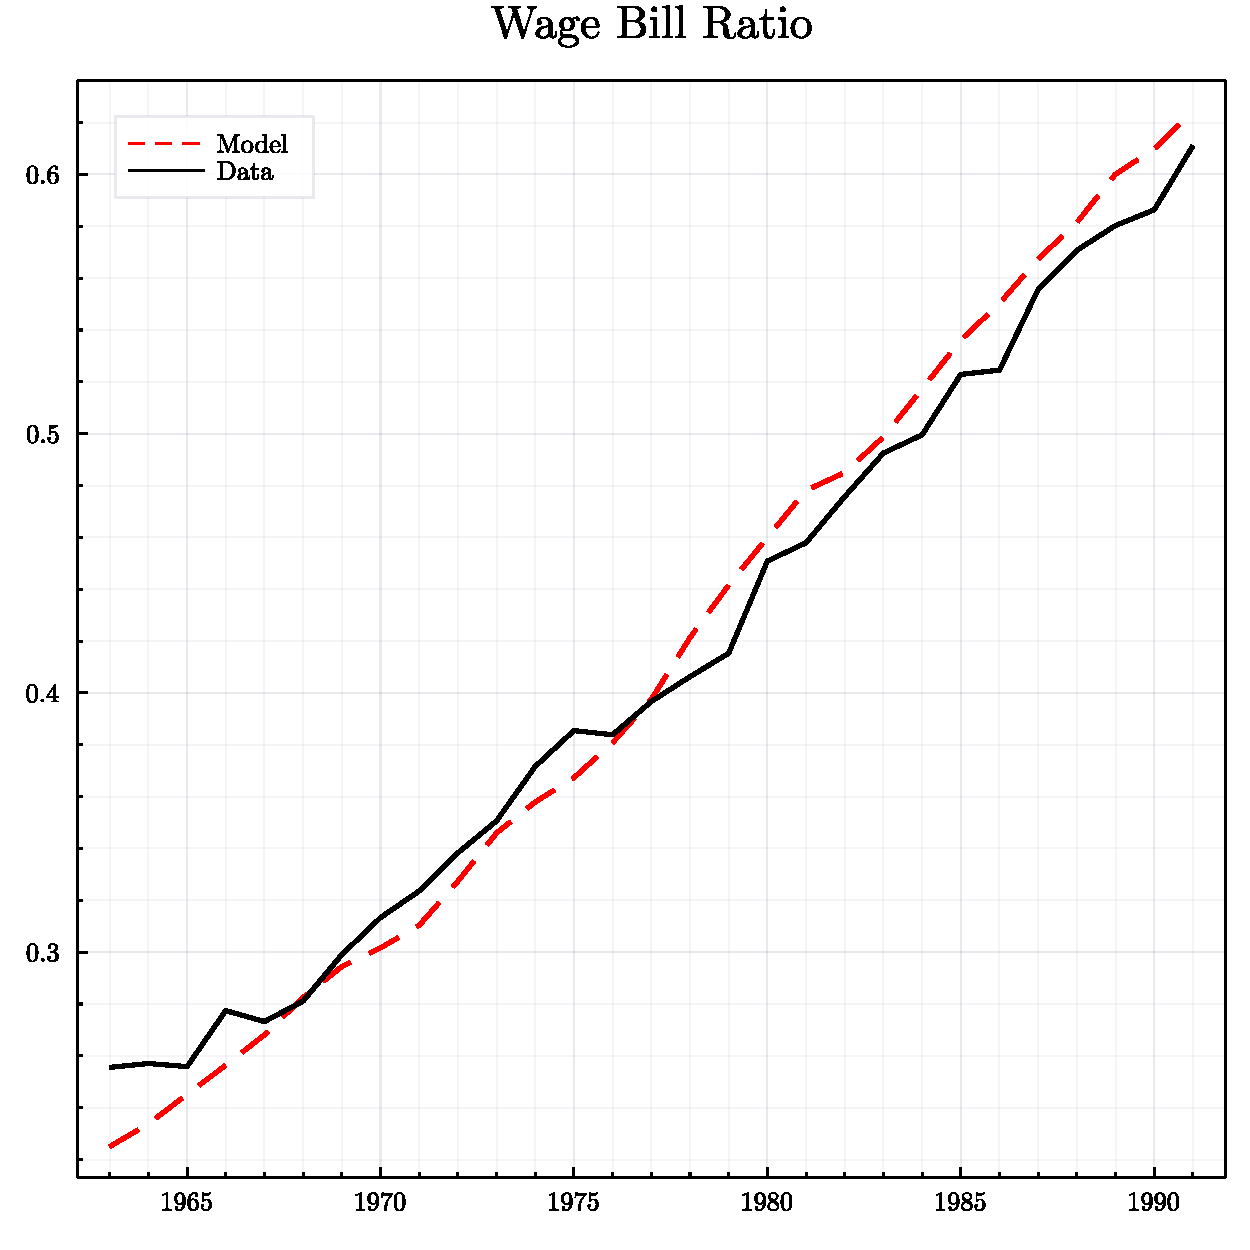
\includegraphics[width=\textwidth]{../images/fig:korv_estimation_wbr_doc.pdf}
  %     \caption{$y=3sinx$}
  %     \label{fig:three sin x}
  % \end{subfigure}
  % \hfill
  % \begin{subfigure}%[b]{0.3\textwidth}
  %     \centering
  %     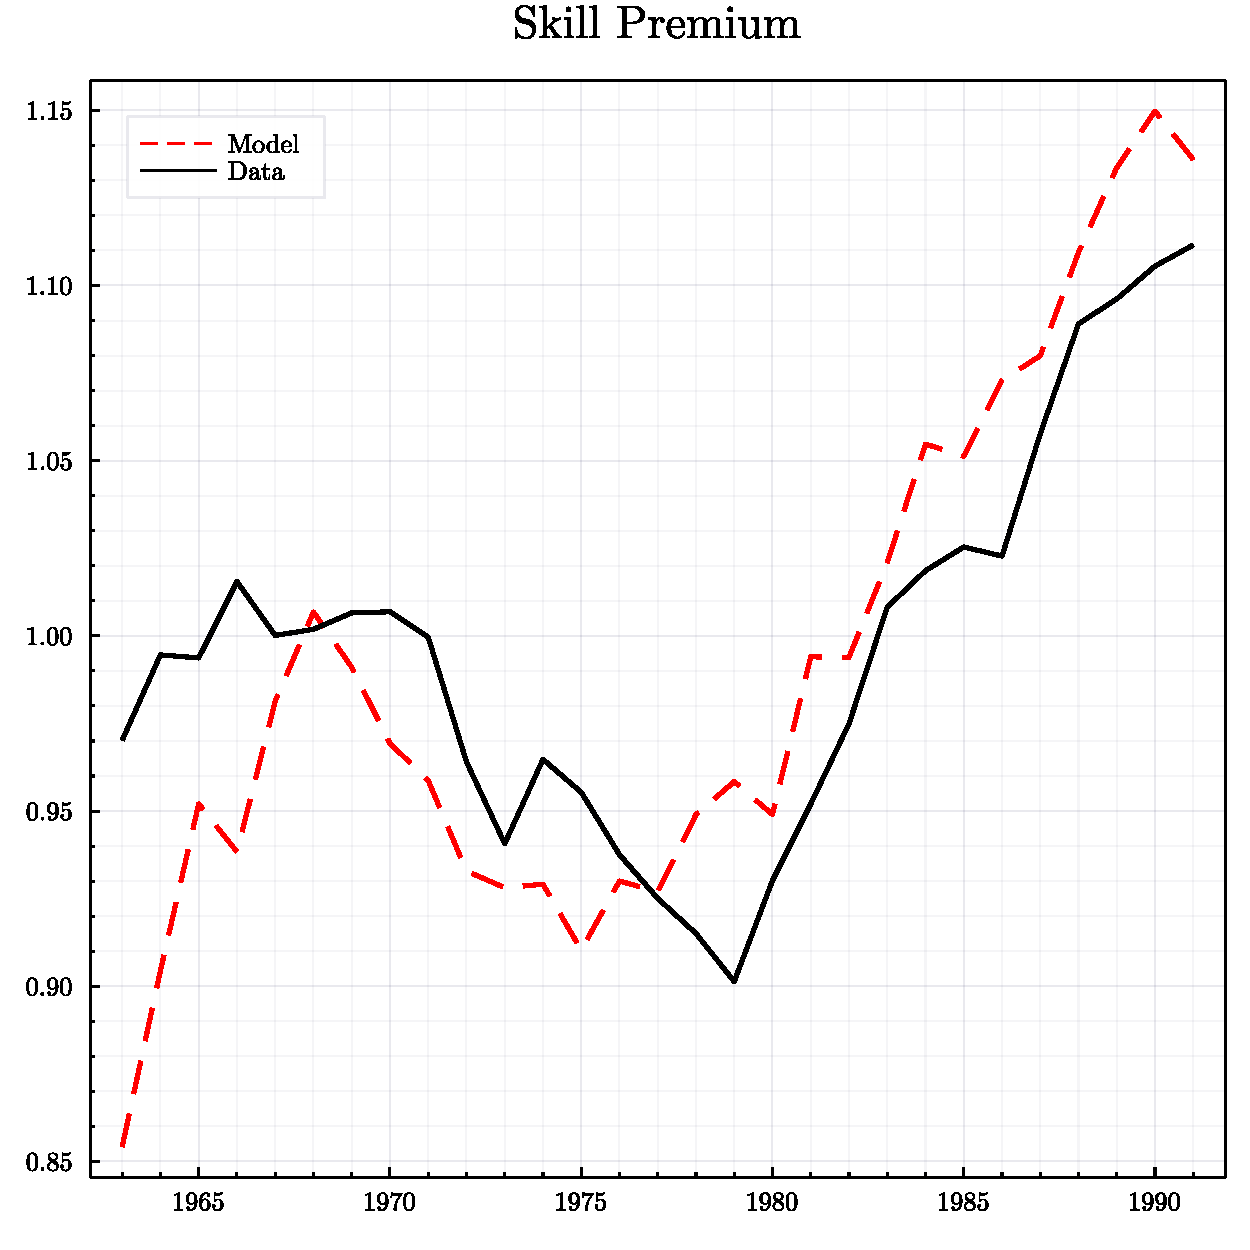
\includegraphics[width=\textwidth]{../images/fig:korv_estimation_sp_doc.pdf}
  %     \caption{$y=5/x$}
  %     \label{fig:five over x}
  % \end{subfigure}
%     \caption{Three simple graphs}
%     \label{fig:three graphs}
% \end{figure}




As seen in table \ref{tab:estimation_korv} \textcolor{red}{Descirbe results}\dots


\subsection{Estimation by Industry}


\pagebreak{}

\bibliographystyle{chicago}
\bibliography{references}

\pagebreak{}

\appendix

\section{Ommited Derivations}\label{sec:derivations}
Outline:
\begin{itemize}
  \item FOC of Labor and Skill premium
  \item Log Linearization
  \item Write it as growth rates
\end{itemize}

\section{Data Construction}\label{sec:data-construction}


\subsection{Capital Inputs and Labor Share}\label{subsec:capital-inputs-labor-share}
OUTLINE
\begin{itemize}
	\item Mention why are those delators used.
	\item How is the depreciation rate contructed?
\end{itemize}

% # After looking up the same for Structures and Intelectual Property I get:
%     # * Stock of Capital:
%     #     - (FAAt301S) Table 3.1S. Current-Cost net Stock of Private Structures by Industry
%     #     - (FAAt301I) Table 3.1I. Current-Cost Net Stock of Intellectual Property Products by Industry
%     # * Investment:
%     #     - (FAAt307S) Table 3.7S. Investment in Private Structures by Industry
%     #     - (FAAt307I) Table 3.7I. Investment in Private Intellectual Property Products by Industry
%     # * Depreciation:
%     #     - (FAAt304S) Table 3.4S. Current-Cost Depreciation of Private Structures by Industry
%     #     - (FAAt304I) Table 3.4I. Current-Cost Depreciation of Private Intellectual Property Products by Industry

\subsection{Labor Inputs and Wage Rates}\label{subsec:labor-inputs-wage-rates}


\end{document}